\documentclass[11pt,a4paper]{article}
\usepackage[margin=24mm]{geometry}
\usepackage[utf8]{inputenc}
\usepackage{tikz}
\usetikzlibrary{positioning}
\title{Derived requirement trace down to procured items}
\date{Created 2026-10-07 14:20 CEST}
\begin{document}
\maketitle
\paragraph{Scope and estimate.} The halfarm model traces requirements to blocks by hand
(\texttt{satisfies}). The user wants the trace carried through the composition to the concrete
procured items, and the result imported into a Mission Control view (another agent's repository).
User decisions 2026-10-07 (answered before 14:20): (1) the model is the source of the 37 procurement lines and the
equipment workbook is generated from it; (2) the derived relation is a separate \texttt{<derived>}
\emph{affects} edge, \texttt{satisfies} stays manual; (3) Mission Control receives a generated
\texttt{.hymeko} module; (4) first step: the 44 NIST/SIL requirements replace R1--R20 in the model.
ETA 4--5 hours. No benchmark.
\paragraph{Semantics.} For each manual \texttt{satisfies} edge $s = (+b, -r)$ two derived n-ary
edges are generated: \emph{down} $= (-r, +x \ldots)$ for every $x$ reachable from $b$ along
composition (whole $\to$ part) and realization (block $\to$ product or node), and \emph{up}
$= (-r, +y\ldots)$ for every composite $y$ containing $b$. Field \texttt{via} names $s$. \emph{Affects}
means ``may be impacted'' (change-impact analysis), not ``satisfies''.
\paragraph{Ownership.} Query: \texttt{rewrite/scope.rs} gains root items
\texttt{bind:<sign>:<index|all>} (the current match's binding targets, so a nested \texttt{\#each}
takes its root from the enclosing match) and source items \texttt{inverse:<label>} (follow
$-\to+$). \texttt{RenderContext} is unchanged (a downstream struct literal in \texttt{hymeko\_web}).
Vocabulary: \texttt{data/sysml/meta\_sysml\_structure.hymeko} gains \texttt{priority\_level} (with
\texttt{rank}, as in the Mission Control program vocabulary), \texttt{safety\_function},
\texttt{standard\_ref}, \texttt{product}, \texttt{@cites} (+ requirement, $-$ standard\_ref\ldots),
\texttt{@affects} (+ element\ldots, $-$ requirement). The standard catalog subset and all model
content live with the consumer (\texttt{02\_design/sze/halfarm/model}).
\paragraph{Tests.} Unit: \texttt{bind:} roots inside a nested \texttt{\#each}, \texttt{bind:+:all},
\texttt{inverse:} sources, mixed sources. Counter-tests: \texttt{bind:} outside any match resolves no
root; \texttt{inverse:} of an unknown label follows nothing; without \texttt{inverse:} a product is not
reached. Consumer: generated requirement table equals the document table (44 rows, every column);
generated workbook equals the previous totals and quantities; derived module compiles with the model,
regenerating it is byte-identical (freshness check), and removing one composition edge changes exactly
the expected derived edges.
\paragraph{Budget and risks.} Closure per satisfies edge: $O(\mathrm{iterations}\times
\mathrm{edge\ matches})$, about 60 satisfies edges on a few hundred matches. Risk: \emph{down}
over-approximates (every part of a composite); it is labelled \emph{affects}, never \emph{satisfies}.
Risk: name resolution of the generated module (cross-file references) -- checked by compiling.
\paragraph{State and rollback.} Checkout on \texttt{feat/material-lobes} with the uncommitted
2026-10-06/07 changes; another worker's files untouched. No git writes from the sandbox. Rollback:
revert the \texttt{scope.rs} hunks and the vocabulary additions; the consumer files are separate.
\begin{center}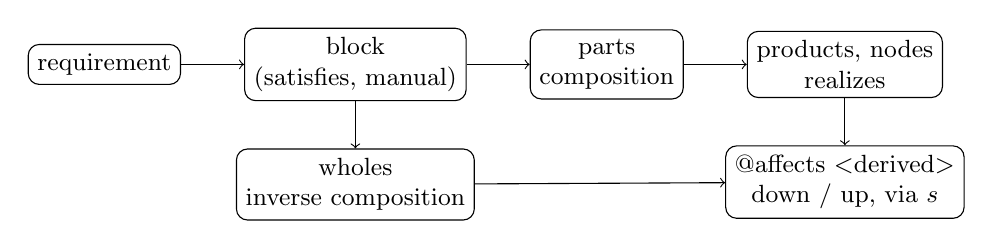
\begin{tikzpicture}[node distance=6mm and 8mm, every node/.style={draw, rounded corners, font=\small, align=center}]
\node (r) {requirement};
\node (b) [right=of r] {block\\(satisfies, manual)};
\node (p) [right=of b] {parts\\composition};
\node (i) [right=of p] {products, nodes\\realizes};
\node (u) [below=of b] {wholes\\inverse composition};
\node (a) [below=of i] {@affects $<$derived$>$\\down / up, via $s$};
\draw[->] (r) -- (b); \draw[->] (b) -- (p); \draw[->] (p) -- (i); \draw[->] (b) -- (u);
\draw[->] (i) -- (a); \draw[->] (u) -- (a);
\end{tikzpicture}
\end{center}
\end{document}
